\documentclass[a4paper,12pt]{article}
\usepackage[utf8]{inputenc}
\usepackage[english]{babel}
\usepackage[T1]{fontenc} % for correct << and >>
\usepackage{amssymb, amsmath, multicol, amsthm, mathtools}
\usepackage{csquotes}
\usepackage{mathrsfs}
\usepackage{graphicx}
\usepackage{multirow}
\usepackage{caption}
\usepackage{subcaption}
\usepackage{indentfirst}
\usepackage{esvect}
\usepackage{float} 
\usepackage[version=4]{mhchem}
\mathtoolsset{showonlyrefs=true}
\usepackage{hyperref}
\usepackage[rgb,table,xcdraw]{xcolor}
\hypersetup{				
	unicode=true,        
	colorlinks=true,       	
	linkcolor=black,        
	citecolor=black,        
	filecolor=magenta,      
	urlcolor=black         
}

\usepackage[left=2cm,right=2cm,
    top=2cm,bottom=2cm]{geometry}
\usepackage{fancyhdr}



\newcommand{\angstrom}{\text{\normalfont\AA}}
\graphicspath{{images}}

\usepackage[math-style=ISO, partial=upright]{unicode-math}

\newcommand{\iu}{\mathrm{i}\mkern1mu}

\begin{document}

\section{Definition of the Hamiltonian}

There is a number of details in the definition of the Heisenberg Hamiltonians, which may cause an incompatibility of the direct results. 
In this paper the main definition is as follows:

\begin{equation}
    \hat{H} = -J \sum_{ij} \hat{\mathbf{S}}_i^T \hat{\mathbf{S}}_j
    \label{eq:hh-main}
\end{equation}
where $J$ is an isotropic exchange parameter. The double counting is present in the Hamiltonian, i.e. both terms $i\rightarrow j$ and $j \rightarrow i$ are present in the sum. 
$\hat{\mathbf{S}}_i$ is a $3\times1$ column vector of the spin operators $(\hat{\mathbf{S}}_i^x, \hat{\mathbf{S}}_i^y, \hat{\mathbf{S}}_i^z)$. 
Index $i$ run over all $N$ sites in the system and index $j$ runs over neighbors for the site $i$. 

Bold mathematical symbols in this work represent vectors or matrices and usual symbols - scalars. For instance, $J$ is a scalar exchange parameter, while $\mathbf{J}$ is a matrix of exchange, 
for the isotropic case it is defined as

\begin{equation}
    \mathbf{J} =
    \begin{pmatrix}
        J & 0 & 0 \\
        0 & J & 0 \\
        0 & 0 & J
    \end{pmatrix}
\end{equation}

Several comparisons of the exchange Hamiltonians and consecutive spin wave Hamiltonians will be done in this paper and for each one the details of the convergence will be discussed. 
When possible the results will be present in both ways: the original source and in the definition of this paper.

\section{Ferromagnetic cubic system}

In this section I will define the parameters and they values for the case study system - 
cubic lattice of ferromagnetic spins oriented along the direction of $z$ axis.

Lattice (see~Fig.~\ref{fig:lattice}) in cartesian coordinate system is defined by the lattice parameters and angles:
\begin{equation}
    \begin{matrix}
        \mathbf{a} = (l, 0, 0) & \mathbf{b} = (0, l, 0) & \mathbf{c} = (0, 0, l) \\
        \alpha = 90^{\circ} & \beta = 90^{\circ} & \gamma = 90^{\circ} \\
    \end{matrix}
\end{equation}
In each unit cell there is one spin $S$ at the position $(0, 0, 0)$ (in relative coordinates).

Spin in the $(0, 0, 0)$ unit cell will have 6 neighbors as shown in Fig.~\ref{fig:lattice-neighbors}.

\begin{figure}[H]
	\centering
	\begin{subfigure}[b]{0.49\textwidth}
		\centering
		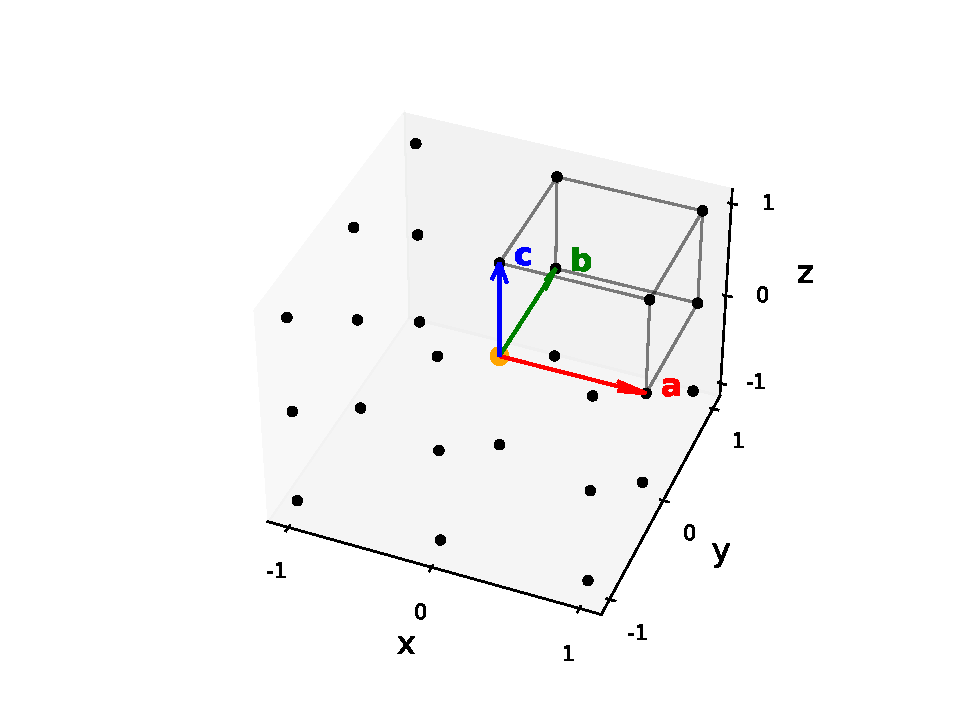
\includegraphics[height=6cm]{lattice.pdf}
        \caption{}
	\label{fig:lattice}
	\end{subfigure}
	\hfill
	\begin{subfigure}[b]{0.49\textwidth}
		\centering
		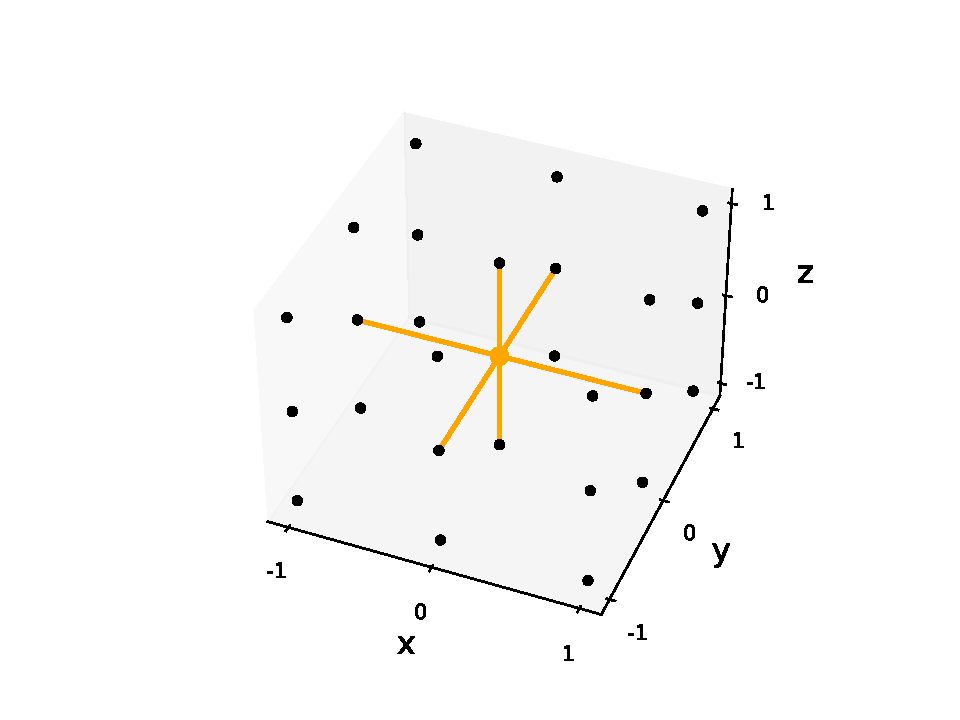
\includegraphics[height=6cm]{lattice-neighbors.pdf}
	\caption{}
	\label{fig:lattice-neighbors}
	\end{subfigure}
	\hfill
	\caption{(a) Lattice and (b) 6 neighbors for the spin in $(0, 0, 0)$ unit cell.}
    \label{fig:lattice-both}
\end{figure}


The reciprocal lattice will have the form of:
\begin{equation}
    \begin{matrix}
        \mathbf{b_1} = (\dfrac{2\pi}{l}, 0, 0) & \mathbf{b_2} = (0,\dfrac{2\pi}{l}, 0) & \mathbf{b_3} = (0, 0, \dfrac{2\pi}{l}) \\
        k_{\alpha} = 90^{\circ} & k_{\beta} = 90^{\circ} & k_{\gamma} = 90^{\circ} \\
    \end{matrix}
\end{equation}

Magnon dispersion plots will use the following path: $\Gamma$-X-M-$\Gamma$-R-X$\vert$M-R (see~Fig.~\ref{fig:path}).

\begin{figure}[H]
	\centering
	\begin{subfigure}[b]{0.8\textwidth}
		\centering
		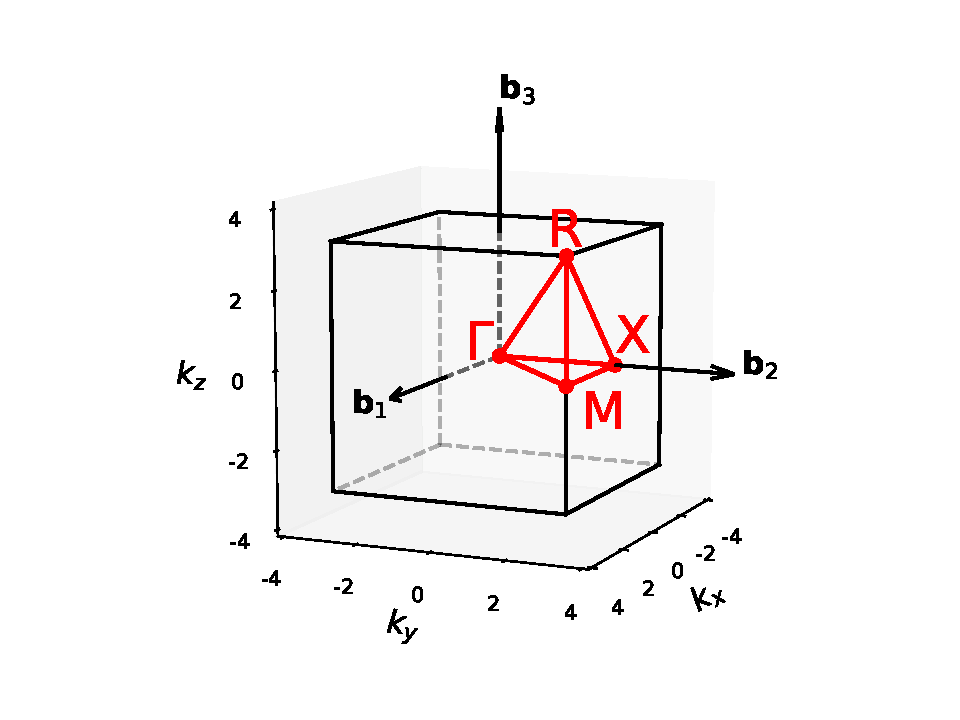
\includegraphics[height=10cm]{path.pdf}
	\end{subfigure}
	\hfill
	\caption{Path in reciprocal space for the magnon dispersion plot: $\Gamma$-X-M-$\Gamma$-R-X$\vert$M-R.}
	\label{fig:path}
\end{figure}


For the final results and for the Figs.~\ref{fig:lattice-both}~and~\ref{fig:path} the following numerical values are used:
\begin{equation}
    \begin{matrix}
        J = 1 \text{ meV}, & S = 1, & l = 1
    \end{matrix}
\end{equation}

\section{Magnon dispersion}

In this section I will derive the magnon dispersion formula from the Hamiltonian~in~\eqref{eq:hh-main}.
First of all I rewrite the Hamiltonian using the raising and lowering spin operators:
\begin{equation}
    \begin{matrix}
        \hat{S}_i^{\pm} = \hat{S}_i^x \pm \iu \hat{S}_i^y \\
        \hat{\mathbf{S}}_i^T \hat{\mathbf{S}}_j = \hat{S}_i^x \hat{S}_j^x + \hat{S}_i^y \hat{S}_j^y + \hat{S}_i^z \hat{S}_j^z \\
        \hat{S}_i^x \hat{S}_j^x + \hat{S}_i^y \hat{S}_j^y = \dfrac{1}{2}\left(
            \hat{S}_i^+\hat{S}_j^- + \hat{S}_i^-\hat{S}_j^+
        \right)
    \end{matrix}
\end{equation}

\begin{equation}
    \hat{H} = -J \sum_{ij} \left(\dfrac{1}{2}\left(
        \hat{S}_i^+\hat{S}_j^- + \hat{S}_i^-\hat{S}_j^+\right) + \hat{S}_i^z \hat{S}_j^z\right)
\end{equation}
since
\begin{equation}
    \left[\hat{S}_i^+\hat{S}_j^-\right] = 2\hat{S}_i^z\deltA_{ij}
\end{equation}
and $i\ne j$ in the sum:
\begin{equation}
    \hat{H} =-J \sum_{ij} \left(\dfrac{1}{2}\left(
            \hat{S}_j^-\hat{S}_i^+ + \hat{S}_i^-\hat{S}_j^+\right) + \hat{S}_i^z \hat{S}_j^z\right)
\end{equation}

From this point the Hamiltonian is treated in the linearised Holstein–Primakoff formalism.

\begin{equation}
    \begin{matrix}
        \hat{S}_i^+ = \sqrt{2S}\hat{a}_i \\
        \hat{S}_i^- = \sqrt{2S}\hat{a}_i^{\dag} \\
        \hat{S}_i^z = S - \hat{a}_i^{\dag}\hat{a}_i
    \end{matrix}
\end{equation}

\begin{equation}
    \hat{H} = -J \sum_{ij} \left(\dfrac{1}{2}\left(
        2S\hat{a}_j^{\dag}\hat{a}_i + 2S\hat{a}_i^{\dag}\hat{a}_j\right) + 
        \left(S - \hat{a}_i^{\dag}\hat{a}_i\right)\left(S - \hat{a}_j^{\dag}\hat{a}_j\right)\right)
\end{equation}

\begin{equation}
    \hat{H} = E_0 + \haT{H}^{(2)} + \dots 
\end{equation}
\begin{equation}
    E_0 = -JS^2Nn 
\end{equation}
\begin{equation}
    \hat{H}^{(2)} = -JS \sum_{ij} \left(\hat{a}_j^{\dag}\hat{a}_i + \hat{a}_i^{\dag}\hat{a}_j - 
    \hat{a}_i^{\dag}\hat{a}_i - \hat{a}_j^{\dag}\hat{a}_j\right)
    \label{eq:quadratic-ham}
\end{equation}
where $N$ is the number of spins in the system, $n$ - number of neighbors for each spin ($6$ in the case of cubic system).
From this point I focus on the quadratic part of the Hamiltonian $\hat{H}^{(2)}$.

In the next step the Fourier transform is used to move from the local operators $\hat{a}_i^{dag}$ and $\hat{a}_i$
to the collective creation and annihilation operators $\hat{a}_k^{\dag}$ and $\hat{a}_k$:
\begin{equation}
    \hat{a}_i = \dfrac{1}{\sqrt{N}}\sum_k e^{\iu\mathbf{k}\mathbf{r}_i} \hat{a}_k 
\end{equation}
\begin{equation}
    \hat{a}_i^{\dag} = \dfrac{1}{\sqrt{N}}\sum_k e^{-\iu\mathbf{k}\mathbf{r}_i} \hat{a}_k^{\dag} 
\end{equation}
\begin{equation}
    \dfrac{1}{N}\sum_i e^{\iu(\mathbf{k} - \mathbf{k}^{\prime})\mathbf{r}_i} = \delta_{kk^{\prime}} 
\end{equation}

By substituting it into eq.~\eqref{eq:quadratic-ham} I get:

\begin{aligned}
    \hat{H}^{(2)}  = -JS \sum_i\sum_j \dfrac{1}{N}\left[
        \left(\sum_k e^{-\iu\mathbf{k}\mathbf{r}_j} \hat{a}_k^{\dag}\right)
        \left(\sum_{k^{\prime}} e^{\iu\mathbf{k^{\prime}}\mathbf{r}_i} \hat{a}_{k^{\prime}}\right)\right. \\
        +
        \left(\sum_k e^{-\iu\mathbf{k}\mathbf{r}_i} \hat{a}_k^{\dag}\right)
        \left(\sum_{k^{\prime}} e^{\iu\mathbf{k^{\prime}}\mathbf{r}_j} \hat{a}_{k^{\prime}}\right)  \\
        -
        \left(\sum_k e^{-\iu\mathbf{k}\mathbf{r}_i} \hat{a}_k^{\dag}\right)
        \left(\sum_{k^{\prime}} e^{\iu\mathbf{k^{\prime}}\mathbf{r}_i} \hat{a}_{k^{\prime}}\right)  \\
        -
        \left.\left(\sum_k e^{-\iu\mathbf{k}\mathbf{r}_j} \hat{a}_k^{\dag}\right)
        \left(\sum_{k^{\prime}} e^{\iu\mathbf{k^{\prime}}\mathbf{r}_j} \hat{a}_{k^{\prime}}\right) \right]
\end{aligned}

Since for each $i$ there is the same pattern of neighbors sum over $j$ does not depend on $i$ and I can move it freely.
Lets define $\mathbf{\delta}_j = \mathbf{r}_j - \mathbf{r}_i$ and rewrite the equation:

\begin{aligned}
    \hat{H}^{(2)}  = -JS \sum_k\sum_{k^{\prime}}\sum_j \left[
        e^{-\iu\boldsymbol{\delta}_j\mathbf{k}}
        \left(\dfrac{1}{N}\sum_ie^{\iu(\mathbf{k^{\prime}}-\mathbf{k})\mathbf{r}_i}\right) 
        \hat{a}_k^{\dag}\hat{a}_{k^{\prime}}\right. \\
        +
        e^{\iu\boldsymbol{\delta}_j\mathbf{k}}
        \left(\dfrac{1}{N}\sum_ie^{\iu(\mathbf{k^{\prime}}-\mathbf{k})\mathbf{r}_i}\right)
         \hat{a}_k^{\dag}\hat{a}_{k^{\prime}}  \\
        -
        \left(\dfrac{1}{N}\sum_ie^{\iu(\mathbf{k^{\prime}}-\mathbf{k})\mathbf{r}_i}\right)
        \hat{a}_k^{\dag}\hat{a}_{k^{\prime}}  \\
        -
        \left.e^{\iu(\mathbf{k^{\prime}}-\mathbf{k})\boldsymbol{\delta}_j}
        \left(\dfrac{1}{N}\sum_ie^{\iu(\mathbf{k^{\prime}}-\mathbf{k})\mathbf{r}_i}\right)
        \hat{a}_k^{\dag}\hat{a}_{k^{\prime}} \right]
\end{aligned}
every equation in round parenthesis is equal to $\delta_{kk^{\prime}}$ and the Hamiltonian becomes
\begin{equation}
    \hat{H}^{(2)} = -JS\sum_k\sum_j\left[e^{-\iu\boldsymbol{\delta}_j\mathbf{k}}
    \hat{a}_k^{\dag}\hat{a}_k
    +
    e^{\iu\boldsymbol{\delta}_j\mathbf{k}}
     \hat{a}_k^{\dag}\hat{a}_k 
    -
    \hat{a}_k^{\dag}\hat{a}_k 
    -
    e^{\iu(\mathbf{k}-\mathbf{k})\boldsymbol{\delta}_j}
    \hat{a}_k^{\dag}\hat{a}_k\right]
\end{equation}
since for each $\boldsymbol{\delta}_j$ there is $-\boldsymbol{\delta}_j$ 
present in the sum over $j$ we can rewrite the Hamiltonian one more time:
\begin{equation}
    \hat{H}^{(2)} = 2JS\sum_k\sum_j\left(\hat{a}_k^{\dag}\hat{a}_k - 
    e^{\iu\boldsymbol{\delta}_j\mathbf{k}}\hat{a}_k^{\dag}\hat{a}_k\right)
\end{equation}
for the cubic system $j$ runs from $1$ to $6$, therefore:
\begin{equation}
    \hat{H}^{(2)} = 2JSn\sum_k\left(1 - \dfrac{1}{n}\sum_j
    e^{\iu\boldsymbol{\delta}_j\mathbf{k}}\right)\hat{a}_k^{\dag}\hat{a}_k = 
    \sum_k \hbar\omega(\mathbf{k})\hat{a}_k^{\dag}\hat{a}_k
\end{equation}

For the cubic system ($l$ - length of the lattice vector):
\begin{align}
    \dfrac{1}{n}\sum_j
    e^{\iu\boldsymbol{\delta}_j\mathbf{k}}  = \dfrac{1}{6}\left((e^{\iu k_x l} + e^{-\iu k_x l}) + 
    (e^{\iu k_y l} + e^{-\iu k_y l}) +
    (e^{\iu k_z l} + e^{-\iu k_z l})\right) \\
    = \dfrac{1}{3}\left(\cos(k_x l) + \cos(k_y l) + \cos(k_z l)\right)
\end{align}
and the final formula for the magnon dispersion looks like
\begin{align}
    \boxed{
    \hbar\omega(\mathbf{k}) = 2JSn\left(1 - 
    \dfrac{1}{3}\left(\cos(k_x l) + \cos(k_y l) + \cos(k_z l)\right)\right)}
    \label{eq:main_dispersion}
\end{align}

\begin{figure}[H]
	\centering
	\begin{subfigure}[b]{0.8\textwidth}
		\centering
		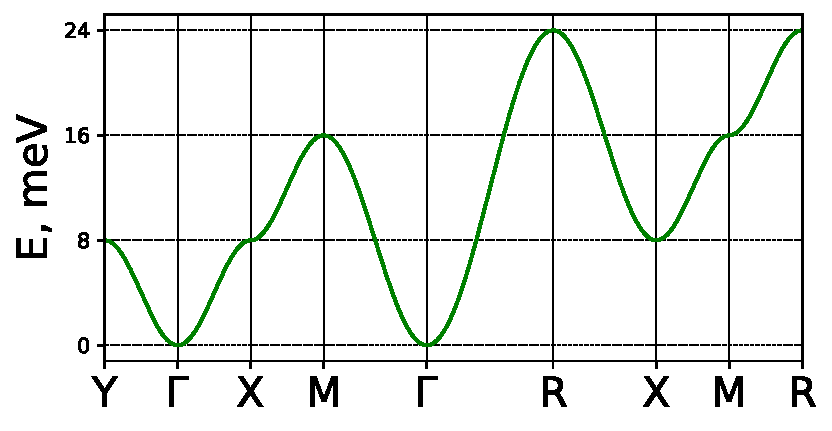
\includegraphics[height=7cm]{main_dispersion.pdf}
	\end{subfigure}
	\hfill
	\caption{Magnon dispersion plotted with equation~\eqref{eq:main_dispersion}.}
	\label{fig:main_dispersion}
\end{figure}




\newpage
\bibliographystyle{plain} 
\bibliography{refs.bib} 
% \section*{References}
% \printbibliography[title = {\vspace{-2em}}]

\end{document}
